


To illustrate how vehicle system works 
and how each components are related to different OBD parameters,
we present a high-level vehicle system control 
flow in Fig. \ref{vehicle_system}. 
Drivers accelerate vehicle by pressing the gas pedal, 
and then the gas pedal position will be sent to 
the Electronic Control Unit (ECU). 
The ECU controls air/fuel injection rate
to produce engine torque to drive the vehicle.   
Transmission is used in this process 
to transit power from engine to wheel and 
match engine rotational speed with wheel rotational speed. 


\begin{figure}[t]
\begin{center}
\vspace{-0.0cm}
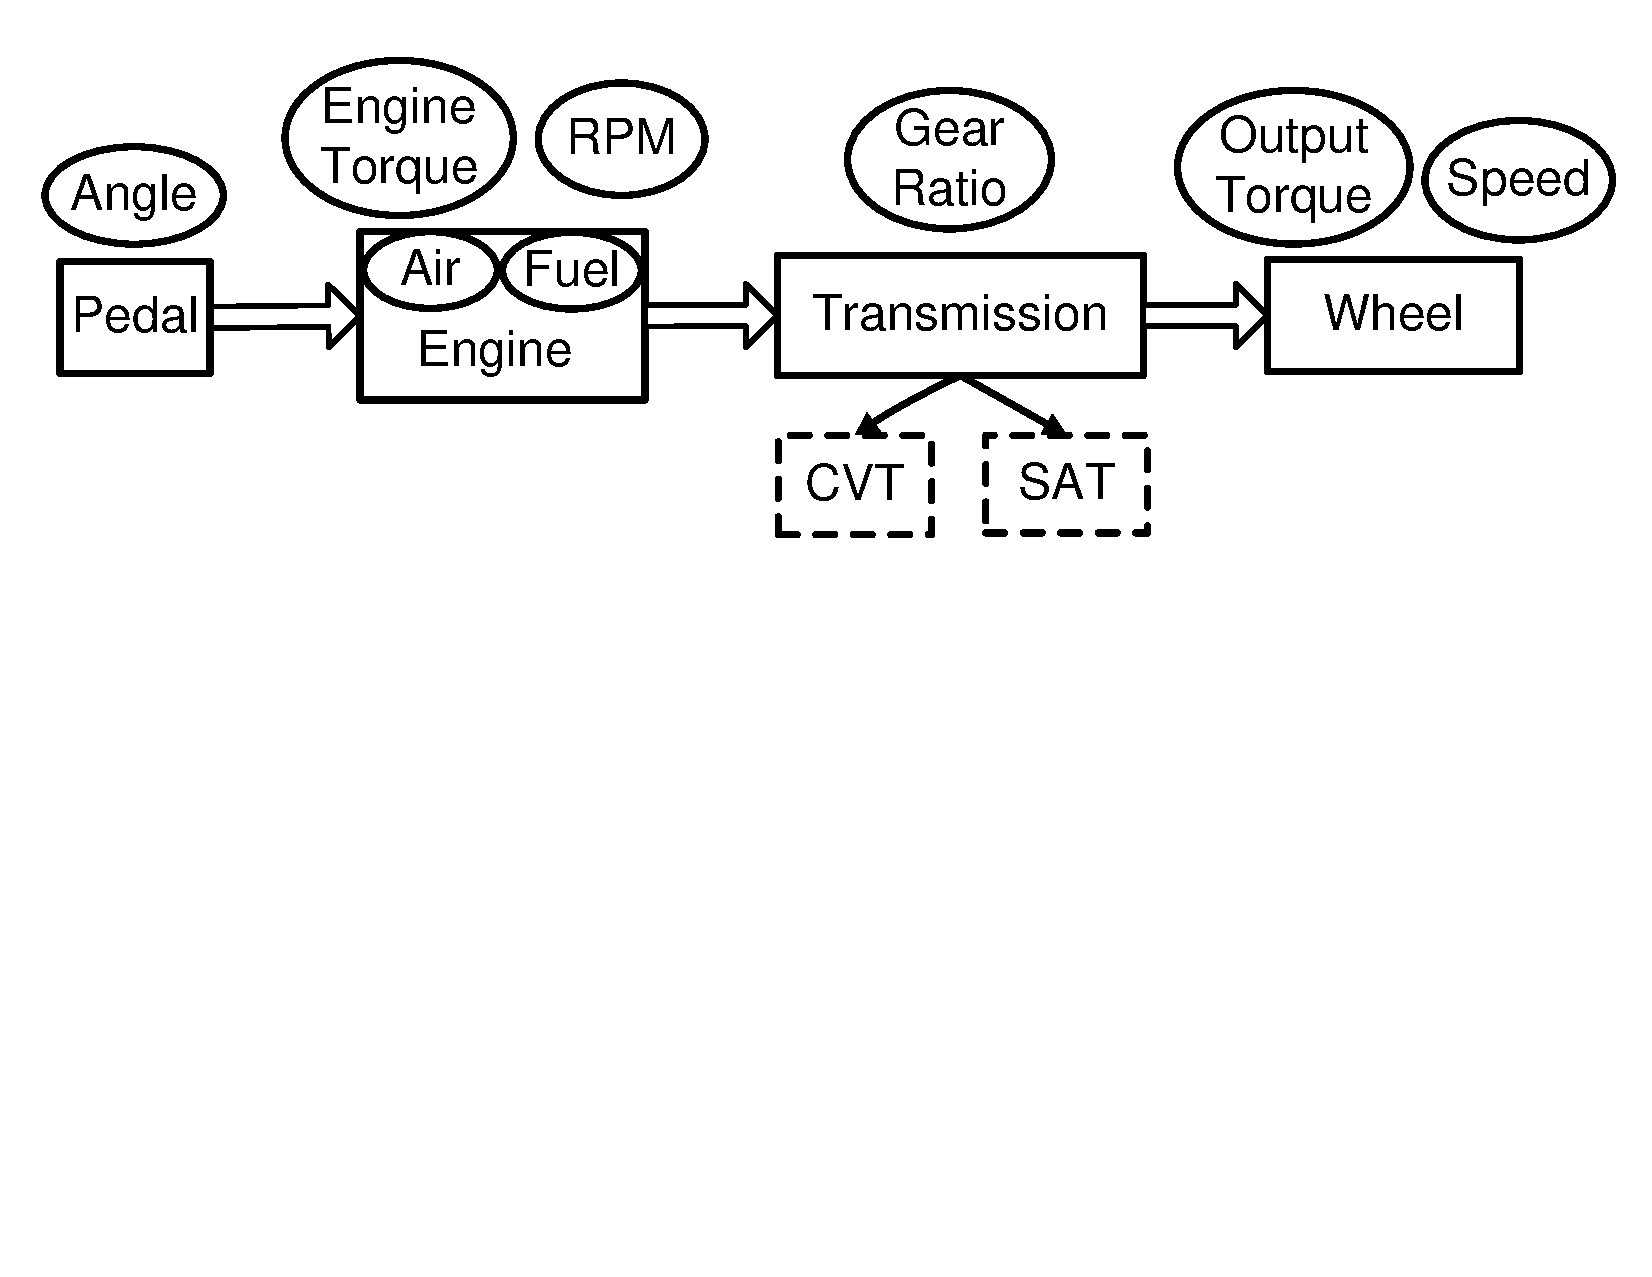
\includegraphics[width=5.0in,angle=0]{Figs/EcoDrive/drivetrain.pdf}
\vspace{-5.5cm}
\caption{Vehicle Drivetrain.}
\vspace{-0.5cm}
\label{vehicle_system}
\end{center}
\end{figure}


\subsection{Power Production and Transition}

In a car engine, the explosion of compressed fuel and air 
produces the power to drive a car.
The air is injected through an intake port and expelled from an exhaust port.
The volume of oxygen in the exhaust air is monitored by fuel trim sensors. 
Based on fuel trim sensor readings, the Electronic Control Unit (ECU) 
calculate the desired fuel injection rate to maintain the
ideal air/fuel ratio 
\footnote{Air/fuel ratio is a constant value around 14.67, 
while air/fuel rate is the volume of air/fuel injected per unit time.}. 


The burning of air and fuel mixture triggers the revolution of 
crankshaft, which carries piston power out of the engine to the transmission.
The transmission carries power to wheels.  
Transmission is also known as gearbox that uses gears and gear trains
to provide speed and torque conversion. 
The transmission reduces the higher engine speed to the slower
wheel speed and increases torque in the process of accelerating the vehicle. 
The transmission converts engine revolutions to driveshaft revolutions, and then to axle revolutions.
A Continuously Variable Transmission (CVT) is a 
transmission that can change 
seamlessly through an infinite number of effective gear ratios 
between maximum and minimum values. 
This contrasts with Step 
Automatic Transmissions (SAT) that offer a fixed number of gear ratios.

\subsection{OBD Parameters}

\begin{table}[!htbp]
        \centering
        \caption[obd_data]{Collected OBD Data}
         \vspace{0.5cm}
        \label{obd_data}
                \begin{tabular}{|l|c|c|}
                \hline
Name & PID & Unit 
\\  \hline      \hline
Fuel Level (FL) & 2F & $\%$     
\\  \hline
Mass Air Flow Rate (MAF) & 10 & g/s   
\\   \hline
Fuel System Status (FSS) & 03  & Bitmask  
\\  \hline
Long Term Fuel Trim (LTFT) & 07  &  $\%$  
\\  \hline
Short Term Fuel Trim (STFT) & 06 &  $\%$  
\\   \hline
Vehicular Speed (VS) &  0D &  km/h   
\\  \hline
Engine RPM (RPM) & 0C & rpm 
\\   \hline
Accelerator Position (AP) & 5A & $\%$  
\\   \hline
      \end{tabular}
\end{table}


On-board diagnostics (OBD) is an automotive 
term referring to a vehicle's 
self-diagnostic and reporting capability.  
It is the interface between car Controller Area Network (or CAN bus) and external devices, 
e.g., a OBD scan tool that connects the OBD port and a laptop. 
Car CAN bus allows vehicular components to communicate with each other. 
For example, a position value is sent to 
the Electronic Control Unit (ECU) after human driver
press the gas pedal, 
and the ECU adjusts air/fuel injections according to the position value.
Therefore, we can read this position message transmitted over CAN bus 
from the OBD port. 





The data we collected from the OBD port are summarized in Table \ref{obd_data}. 
Fuel Level (FL) of the vehicle is usually measured by a float sensor, 
which is usually visualized on the fuel gauge in the car \cite{fuel-gauge}.
The FL is calculated according to the height of the float. 
\nop{
When fuel is injected into the tank, the fuel will raise 
the float up, and vice versa. 
This mechanism makes the FL measurement is not accurate
and can be only used to long-term fuel consumption estimation. 
For example, the float may reach the top of the tank even 
before the tank is filled up.
The fuel gauge will show a full tank even 
when more fuel is possible to be filled.  
Similar thing happens when the fuel tank close to empty. 
}
The Fuel System Status (FSS) is used to indicate current engine mode, 
open loop mode or closed loop mode. 
In open loop mode, 
the engine calculate the fuel injection based on the pre-calculated
table and there is no feedback to the engine to adjust the fuel injection rate. 
The engine runs in open loop mode during short warm up time
and runs in closed loop mode at most of the time. 
In closed loop mode, the engine adjusts fuel injection rate based on
fuel trims and air flow rate. 
Mass Air Flow Rate (MAF) is used to measure the air intake rate of the engine, 
and therefore an effective indicator of instant fuel consumption 
\cite{alessandrini2012consumption, lee2011estimation, koukoumidis2011signalguru}. 
Both Long Term Fuel Trim (LTFT) and Short Term Fuel Trim (STFT) are used to 
adjust the air/fuel rate injected into engine. 
LTFT changes less frequent than STFT. 
We use AFR as a metric of 
instant fuel consumption and/or carbon emission. 


\begin{equation}
AFR = C_f * MAF * (1 + LTFT) * (1 + STFT).
\end{equation}

where $C_f$ is a constant value for unit conversion, e.g., from air flow rate to
fuel rate or to carbon emission rate. 

Vehicular Speed is measured by the perimeter of the wheel and 
number of rotations. 
Accelerator Position is measured by the angle of the gas pedal.
It controls the air/fuel rate injected into the Engine.  
Engine RPM is measured by the rotation speed of the engine motor. 


\subsection{Dataset}


\begin{table}[t]
        \centering
        \caption[vehicles]{Vehicles (distance in miles)}
         \vspace{0.5cm}
        \label{vehicles}
                \begin{tabular}{|c|c|c|c|c|c|}
                \hline
No. & Car Model  & Urban & Highway  
\\  \hline      \hline
%lei
1  & Chevrolet Impala 2011 &  1051   &  852
\\  \hline
%bozhao
2 & Nissan Rogue 2011   &  1198 &  1063 
\\   \hline
%xun zhao
3 & Subaru Forester 2011 & 651  & 757
\\   \hline
%jianqiao
4  &Buick LaCrosse 2006 & 599  & 649 
\\   \hline
%ling zheng
5  & Volkswagen Tiguan 2014  & 600  & 347 
\\   \hline
%zhubo
6 & Honda Accord  2013 & 173 & 840
\\   \hline
%lixing
7 & Toyota Camry 2011    & 35  &  338
\\   \hline
%hao wu
8  & Volkswagen Touareg 2014  & 21  & 156 
\\   \hline
%altima
9 & Nissan Altima 2014  & 193 & 271
\\ \hline
%zhen yang
10 & Nissan Rogue 2011   & 105  &  0 
\\ \hline
%rho
11 & Subaru Legacy 2015 & 119 & 30
\\   \hline
%yangsong
12 & Mazda CX5 2014 & 202  & 89
\\   \hline
    \end{tabular}
\end{table}


\nop{
\begin{table*}[t]
        \centering
        \caption[vehicles]{Vehicles used to collect OBD data}
         \vspace{0.5cm}
        \label{vehicles}
                \begin{tabular}{|c|c|c|c|c|c|}
                \hline
No. & Car Make and Model & Year & Transmission Type  & Urban Miles & Highway Miles  
\\  \hline      \hline
%lei
1  & Chevrolet Impala & 2011 & SAT &  1051   &  852
\\  \hline
%bozhao
2 & Nissan Rogue & 2011 & CVT   &  1198 &  1063 
\\   \hline
%xun zhao
3 & Subaru Forester & 2011 & SAT  & 651  & 757
\\   \hline
%jianqiao
4  &Buick LaCrosse & 2006 & SAT  & 599  & 649 
\\   \hline
%ling zheng
5  & Volkswagen Tiguan & 2014 & SAT  & 600  & 347 
\\   \hline
%zhubo
6 & Honda Accord  & 2013  &  CVT & 173 & 840
\\   \hline
%lixing
7 & Toyota Camry & 2011 & SAT   & 35  &  338
\\   \hline
%hao wu
8  & Volkswagen Touareg & 2014 & SAT  & 21  & 156 
\\   \hline
%altima
9 & Nissan Altima & 2014 & CVT & 193 & 271
\\ \hline
%zhen yang
10 & Nissan Rogue & 2011 & CVT   & 105  &  0 
\\ \hline
%rho
11 & Subaru Legacy & 2015  & CVT & 119 & 30
\\   \hline
%yangsong
12 & Mazda CX5 & 2014 & SAT & 202  & 89
\\   \hline
    \end{tabular}
\end{table*}
}


\begin{figure}[t]
\begin{center}
%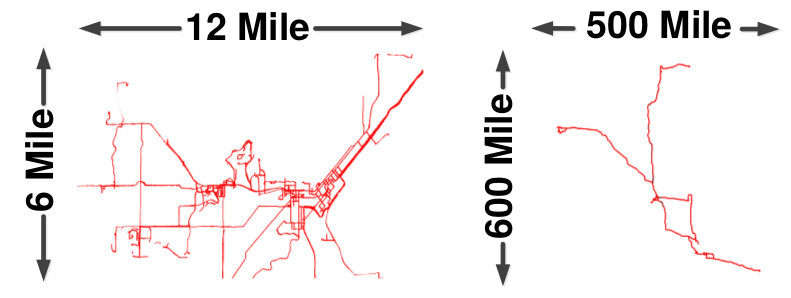
\includegraphics[width=3.0in, angle=0]{Figs/EcoDrive/urbanhighwaymap.png}
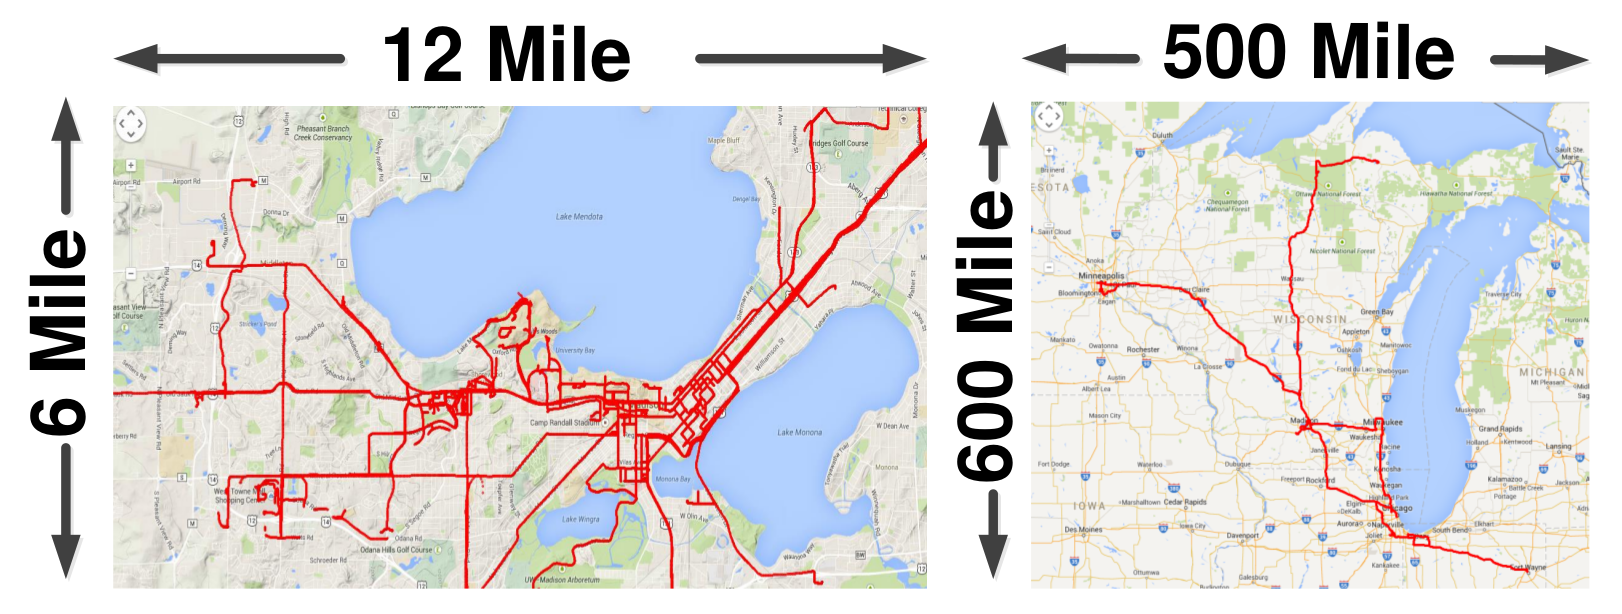
\includegraphics[width=5.0in, angle=0]{Figs/EcoDrive/map.png}
\vspace{-0.0cm}
\caption{Urban driving data (left) is collected from a US mid-size city.  
Highway driving data (right) is collected from both local highways and cross-state highways.}
\vspace{-0.5cm}
\label{rpm_gph}
\end{center}
\end{figure}


%The map area is about 600 mile $\times$ 500 mile.
%The map area is about 6 mile $\times$ 12 mile. 


We use a customized Android application to collect OBD and GPS data 
from different car makes and models.
The dataset is summarized in table \ref{vehicles}.
The transmission of car 2,6,9,10 and 11 is CVT and the rest is SAT. 
The driving data of car 1-6 is collected over a course of three months, 
and the rest is collected from random events, 
e.g., three cross-state highway trips are collected by car 7, 8 and 9, 
respectively. 
Here we separate urban driving and highway driving,
as urban driving patterns are dominated by frequent 
accelerations and decelerations while 
highway driving patterns are dominated by 
constant speed cruising. 
The dataset covers car makes from three different countries, 
urban data over 5,000 miles, highway data across 5 US states and 
over 5,000 miles, two common types of transmissions. 
We use the first car to install a prototype of EcoDrive and tested
it in both urban and highway environments. 
%EcoDrive is tested on Madison's West Betline Highway, between exit 257 and 261. And US 14 Highway between exit 132 and 136.




\subsection{EcoDrive Architecture}

EcoDrive reads real-time OBD parameters through OBD port
and controls air/fuel injection rate by emulating the gas pedal.
We illustrate the architecture of EcoDrive in Fig. \ref{ecodrive}.
The sensed parameters from OBD port are passed to modeling component
to train the models.
The modeling component builds an AFR profile to 
record the instant fuel consumptions of various 
accelerations at different speeds.
Based on pre-calculated driving strategy and real-time sensed vehicular speed, 
the controlling component controls air/fuel injection rate to adjust vehicular speed by 
sending the gas pedal position values to the ECU. 
To emulate the gas pedal, we utilize the drive-by-wire technology, 
where the gas pedal and throttle are connected by electronic messaging instead of mechanical linkage.   
It enables the position of gas pedal can be sent as a message
to control throttle position. 
The throttle controls the volume of air flow injected into the engine. 
 


\subsection{Applications}

EcoDrive is used as an independent system that can be installed
on regular vehicles.  
It can be used as a control system in a way similar to 
cruise control \cite{cruise_control, bengtsson2001adaptive, ioannou1993autonomous}. 
In this application, it is used as a EcoDrive mode that a human driver
can switch it on or off. 
Drivers are required to press the brake pedal to turn this mode off
to keep safe distance to front car or traffic lights/signs accordingly.
This mode can be integrated with intelligent front object or traffic light detection
systems \cite{bengtsson2001adaptive, ioannou1993autonomous} 
to further enhance driving experience. 
EcoDrive requires two inputs, the speed limit and road length. 
The speed limit can be specified by human driver or obtained from online database \cite{speedlimit}. 
The road length can be calculated by a navigation software.



It can also be used as a subsystem of autonomous driving systems 
\cite{googledriverlesscar, urmson2008autonomous, litman2013autonomous, kim2013towards}. 
We envision a highly autonomous and intelligent system that all the route
information are pre-calculated, e.g., speed limit, traffic conditions and
distances of each road segment etc. 
EcoDrive can be used as a subsystem to predict fuel consumption
of possible routes \cite{ganti2010greengps} and 
calculate the optimal driving strategy.  



